\documentclass{article}
\pagestyle{myheadings}

\usepackage{fancyhdr}
\pagestyle{fancy}
\lhead{}
\chead{}
\rhead{}
\lfoot{}
\cfoot{}
\rfoot{\normalsize\thepage}
\renewcommand{\headrulewidth}{0pt}
\renewcommand{\footrulewidth}{0pt}
\newcommand{\RomanNumeralCaps}[1]
    {\MakeUppercase{\romannumeral #1}}

\usepackage{amssymb,latexsym}  % Standard packages
\usepackage[utf8]{inputenc}
\usepackage[russian]{babel}
\usepackage{MnSymbol}
\usepackage{mathrsfs}
\usepackage{amsmath,amsthm}
\usepackage{indentfirst}
\usepackage{graphicx}%,vmargin}
\usepackage{epigraph}
\usepackage[all]{xy} %для XyPic'a
\usepackage{hyperref}
\usepackage{color}
\usepackage{tikz}

\newtheorem{Lemma}{Лемма}[section]
\newtheorem{Proposition}{Предложение}[section]
\newtheorem{Theorem}{Теорема}[section]
\newtheorem{Corollary}{Следствие}[section]
\newtheorem{Remark}{Замечание}[section]
\newtheorem{Definition}{Определение}[section]
\newtheorem{Designations}{Обозначение}[section]


\usepackage{tocloft}
\renewcommand{\cfttoctitlefont}{\hspace{0.38\textwidth} \huge\bfseries\MakeUppercase}
\renewcommand{\cftbeforetoctitleskip}{-1em}
\renewcommand{\cftaftertoctitle}{\mbox{}\hfill \\ \mbox{}\hfill{\footnotesize Стр.}\vspace{-0.5em}}
%\renewcommand{\cftchapfont}{\normalsize\bfseries \MakeUppercase{\chaptername} }
\renewcommand{\cftsecfont}{\hspace{1pt}}
\renewcommand{\cftsubsecfont}{\hspace{1pt}}
%\renewcommand{\cftbeforechapskip}{1em}
\renewcommand{\cftparskip}{3mm} %определяет величину отступа в оглавлении
\renewcommand{\cftdotsep}{1} %частота точек
\setcounter{tocdepth}{3}

%%%%%%%Запиливание переопределённого chapter в оглавление%%%%%%
\makeatletter
\renewcommand{\@dotsep}{2}
\newcommand{\l@likechapter}[2]{{\bfseries\@dottedtocline{0}{0pt}{0pt}{#1}{#2}}}
\makeatother
\newcommand{\likechapter}[1]{
\likechapterheading{#1}
\addcontentsline{toc}{likechapter}{\MakeUppercase{#1}}}

\addtolength{\textwidth}{0.7in}
\textheight=630pt
\addtolength{\evensidemargin}{-0.4in}
\addtolength{\oddsidemargin}{-0.4in}
\addtolength{\topmargin}{-0.4in}


%%%%%%%%%%%%%%%%%%%%%%%%%%%%%
%%%%%%главы -- section*%%%%%%
%%%%section -- subsection%%%%
%subsection -- subsubsection%
%%%%%%%%%%%%%%%%%%%%%%%%%%%%%
\def \newstr {\medskip \par \noindent}



\begin{document}
\thispagestyle{empty}
\begin{center}
\rule[0.5ex]{\linewidth}{2pt}\vspace*{-\baselineskip}\vspace*{3.2pt}
\rule[0.5ex]{\linewidth}{1pt}\\[\baselineskip]
{\huge \sc Конспект по математическому}\\[4mm]
{\huge \sc анализу для первого курса}\\[4mm]
\rule[0.5ex]{\linewidth}{1pt}\vspace*{-\baselineskip}\vspace{3.2pt}
\rule[0.5ex]{\linewidth}{2pt}\\
\vspace{6.5mm}

\vspace{4mm}
{\large СПбПУ, ИПММ\\
\smallskip
\smallskip
\textsc{Бакалавриат "Математика и CS"}}\\

\vspace{6.5mm}
{\large\textsc{Лекции Моисеева А. А.}}\\
\vspace{5mm}

\vspace{20mm}

\end{center}
\author{Я}
\begin{center}
\vfill {\large\textsc{Санкт-Петербург}}\\
 \today
\end{center}

\newpage
\tableofcontents{}
\documentclass{article}
\pagestyle{myheadings}

%%%%%%%%%%%%%%%%%%%
% Packages/Macros %
%%%%%%%%%%%%%%%%%%%
\usepackage{mathrsfs}


\usepackage{fancyhdr}
\pagestyle{fancy}
\lhead{}
\chead{}
\rhead{}
\lfoot{}
\cfoot{} 
\rfoot{\normalsize\thepage}
\renewcommand{\headrulewidth}{0pt}
\renewcommand{\footrulewidth}{0pt}
\newcommand{\RomanNumeralCaps}[1]
    {\MakeUppercase{\romannumeral #1}}

\usepackage{amssymb,latexsym}  % Standard packages
\usepackage[utf8]{inputenc}
\usepackage[russian]{babel}
\usepackage{MnSymbol}
\usepackage{mathrsfs}
\usepackage{amsmath,amsthm}
\usepackage{indentfirst}
\usepackage{graphicx}%,vmargin}
\usepackage{epigraph} %%% to make inspirational quotes.
\usepackage[all]{xy} %для XyPic'a
\usepackage{hyperref}
\usepackage{color} 
\usepackage{amscd} %для коммутативных диграмм

%\renewcommand{\baselinestretch}{1.5}
%\sloppy
%\usepackage{listings}
%\lstset{numbers=left}
%\setmarginsrb{2cm}{1.5cm}{1cm}{1.5cm}{0pt}{0mm}{0pt}{13mm}


\newtheorem{Lemma}{Лемма}[section]
\newtheorem{Proposition}{Предложение}[section]
\newtheorem{Theorem}{Теорема}[section]
\newtheorem{Corollary}{Следствие}[section]
\newtheorem{Remark}{Замечание}[section]
\newtheorem{Definition}{Определение}[section]
\newtheorem{Designations}{Обозначение}[section]




%%%%%%%%%%%%%%%%%%%%%%%% 
%Сношение с оглавлением% 
%%%%%%%%%%%%%%%%%%%%%%%% 
\usepackage{tocloft} 
\renewcommand{\cfttoctitlefont}{\hspace{0.38\textwidth} \huge\bfseries\MakeUppercase} 
\renewcommand{\cftbeforetoctitleskip}{-1em} 
\renewcommand{\cftaftertoctitle}{\mbox{}\hfill \\ \mbox{}\hfill{\footnotesize Стр.}\vspace{-0.5em}} 
%\renewcommand{\cftchapfont}{\normalsize\bfseries \MakeUppercase{\chaptername} } 
\renewcommand{\cftsecfont}{\hspace{1pt}} 
\renewcommand{\cftsubsecfont}{\hspace{1pt}} 
%\renewcommand{\cftbeforechapskip}{1em} 
\renewcommand{\cftparskip}{3mm} %определяет величину отступа в оглавлении
\renewcommand{\cftdotsep}{1} %частота точек

\setcounter{tocdepth}{3} 

%%%%%%Переопределение chapter%%%%%% 
\newcommand{\empline}{\mbox{}\newline} 
\newcommand{\likechapterheading}[1]{ 
\begin{center} 
\textbf{\MakeUppercase{#1}} 
\end{center} 
\empline} 

%%%%%%%Запиливание переопределённого chapter в оглавление%%%%%% 
\makeatletter 
\renewcommand{\@dotsep}{2} 
\newcommand{\l@likechapter}[2]{{\bfseries\@dottedtocline{0}{0pt}{0pt}{#1}{#2}}} 
\makeatother 
\newcommand{\likechapter}[1]{ 
\likechapterheading{#1} 
\addcontentsline{toc}{likechapter}{\MakeUppercase{#1}}} 


   
%\renewcommand{\thelikesection}{(\roman{likesection})}
%%%%%%%%%%%
% Margins %
%%%%%%%%%%%
\addtolength{\textwidth}{0.7in}
\textheight=630pt
\addtolength{\evensidemargin}{-0.4in}
\addtolength{\oddsidemargin}{-0.4in}
\addtolength{\topmargin}{-0.4in}


%%%%%%%%%%%%{\arabic{l@likesection}}
% Document %
%%%%%%%%%%%%

%%%%%%%%%%%%%%%%%%%%%%%%%%%%%
%%%%%%главы -- section*%%%%%%
%%%%section -- subsection%%%%
%subsection -- subsubsection%
%%%%%%%%%%%%%%%%%%%%%%%%%%%%%
\def \newstr {\medskip \par \noindent} 



\begin{document}
\thispagestyle{empty}
\begin{center} 
\rule[0.5ex]{\linewidth}{2pt}\vspace*{-\baselineskip}\vspace*{3.2pt} 
\rule[0.5ex]{\linewidth}{1pt}\\[\baselineskip] 
{\huge \sc Конспект по математическому}\\[4mm] 
{\huge \sc анализу для первого курса}\\[4mm] 
\rule[0.5ex]{\linewidth}{1pt}\vspace*{-\baselineskip}\vspace{3.2pt} 
\rule[0.5ex]{\linewidth}{2pt}\\ 
\vspace{6.5mm} 
 
\vspace{4mm} 
{\large СПбПУ, Институт ИПММ\\ 
\smallskip
\smallskip
\textsc{Бакалавриат "Математика и CS"}}\\ 

\vspace{6.5mm} 
{\large\textsc{Лекции Моисеева Алексея Александровича}}\\ 
\vspace{5mm} 

\vspace{20mm} 

\end{center} 
\author{Я}
\begin{center}
\vfill {\large\textsc{Санкт-Петербург}}\\ 
 \today
\end{center}
%%%%%%%%%%%%%%%%%%%%%%%%%%%%%%%%%%%%%%%%%%%%%%%%%%%%%%%%%%%%%%%%%%%%%%%%%%%%%%%%%%%%%%%%%%%%%%
%\ \\[4cm]

%\begin{center}
%\LARGE Конспект по математическому анализу за первый семестр бакалавриата "Математика и CS" %\quad СПбГПУ (лекции Моисеева Алексея Александровича)
%\end{center}

%\ \\[11cm]

%by Плаксин Д.А.
%\rm
%%%%%%%%%%%%%%%%%%%%%%%%%%%%%%%%%%%%%%%%%%%%%%%%%%%%%%%%%%%%%%%%%%%%%%%%%%%%%%%%%%%%%%%%%%%%%%

\newpage

\tableofcontents{}

\newpage
\pagestyle{plain}
\begin{center}
\large \bf Упоминаемая литература
\end{center}

\smallskip

\begin{enumerate}
\item А.П.Аксёнов "Математический анализ, часть 1"
\item В.М.Зорич "Математический анализ, часть 1"
\item Б.П.Демидович "Сборник задач и упражнений по математическому анализу"
\end{enumerate}

\newpage 
\begin{center}

\smallskip
\smallskip
\smallskip
\smallskip

\section{\LARGE{\bf Введение}}


\end{center}

\epigraph{\textit{Будет солнечно или мы пойдём на лекцию?}}
{-- Моисеев А.А.}

\subsection{Логическая символика}

\begin{itemize}
\item Операция $"\neg"$ называется отрицанием и, если $A$ -- суждение, то $\neg A$ есть отрицание этого суждения.
\item Операция $"\vee"$ называется дизъюнкцией, и под $A \vee B$(\textit{читается $"A$ или $B"$}) подразумевается, что выполнено хоть одно из суждений $A$ или $B.$

\item Операция $"\&"$ $("\wedge")$ называется конъюнкцией и $A\;\&\;B("A$ и $B")$ значит что имеют место быть оба высказывания $A$ и $B$ одновременно.

\item Символ $"\Rightarrow"$ называется импликацией и запись $A \Rightarrow B$ изначает, что из высказывания $A$ следует высказывание $B,$ при этом $B$ есть необходимое условия для $A$, а $A$ является достаточным условием для $B.$

\item Символ $"\Leftrightarrow"$ называется равносильностью и $A \Leftrightarrow B$ значит, что для высказывания $A$ необходимо и достаточно условие $B.$

\item Квантор всеобщности $\forall$ читается как $"$для любого/для всякого$"$ и означает, соответственно, то же самое.

\item Квантор существования $\exists$ читается как $"$существует/найдётся$"$.
\end{itemize}

{\bf Важные соотношения:}

\begin{enumerate}
\item $\neg(A\vee B) \Leftrightarrow \neg A \& \neg B$
\item $\neg(A\;\&\; B)\Leftrightarrow \neg A\vee\neg B$
\item $A \Rightarrow B  \Leftrightarrow \neg A\Rightarrow\neg B$
\item $A\Rightarrow B  \Leftrightarrow\neg A\vee B$
\item $\neg \left(\forall x\right) P(x) \Leftrightarrow \exists x \;\;\neg P(x)$
\item $\neg \left(\exists x\right) P(x) \Leftrightarrow \forall x \;\;\neg P(x)$
\end{enumerate}

\subsection{Множества и операции над ними}

\begin{Definition}
Множество -- первичное понятие, обозначается заглавной буквой. Множества состоят из элементов(определённых и хорошо различимых [определение по Кантору]).
\end{Definition}

Если элемент $x$ принадлежит множеству $A,$ тогда это записывается как $x\in A$ и читается $"x$ принадлежит/из $A".$

Аналогично $y\notin A.$

Множество полностью определяется своими элементами. Два множества являются равными тогда и только тогда, когда все их элементы совпадают.\\ $A=B \Leftrightarrow \forall x\;\; x\in A \Rightarrow x\in B.$

\begin{itemize}
\item {\bf Отношение включения}\\
$A\subseteq B$ \textit{ ("$A$ включено в $B$")} $\Leftrightarrow \forall x\;\; x\in A \Rightarrow x\in B.$

\item {\bf Объединение множеств}\\
Пусть $A, B$ -- множества. Тогда множество $C=\{x\mid x\in A \vee x\in B\}$ называется объединением множеств $A$ и $B$ и записывается $C=A\cup B.$

\item {\bf Пересечение множеств}\\
Пусть $A, B$ -- множества. Тогда множество $C=\{x\mid x\in A\;\&\; x\in B\}$ называется пересечением множеств $A$ и $B$ и обозначается $C=A\cap B.$\\
\\Заметим, что если $A$ и $B$ не имеют общих элементов, то тогда их пересечение равно пустому множеству: $C=A\cap B=\varnothing.$
\end{itemize}

Операции объединения и пересечения коммутативны и ассоциативны и связаны между собой дистрибутивными законами.
$$\left(A\cup B\right)\cap C = \left(A\cap B\right)\cup\left(B\cap C\right)$$
$$\left(A\cap B\right)\cup C = \left(A\cup B\right)\cap\left(B\cup C\right)$$
\begin{proof}
Докажем первое равенство. \\
Покажем, что если $x$ принадлежит $\left(A\cup B\right)\cap C$, то $x$ принадлежит $\left(A\cap B\right)\cup\left(B\cap C\right).$ Пусть $x\in \left(A\cup B\right)\cap C,$ тогда $x\in \left(A \cup B\right) \;\&\;x\in C$, отсюда $\left( x\in A \vee x\in B\right) \;\&\; x\in C = 
\\=\left(x\in A \;\&\; x\in C\right) \vee \left(x\in B \;\&\; x\in C\right) = \left(A\cap B\right)\cup\left(B\cap C\right),$ по дистрибутивному свойству операций $\vee,\&.$\\
Второе неравенство доказывается аналогично.
\end{proof}
\subparagraph{Кое-какие свойства}
\begin{enumerate}
\item $A\cup B = A \Leftrightarrow B\subseteq A$
\begin{proof}
$\Rightarrow:$
\\Возьмём элемент из $B.$ Докажем, что он принадлежит $A.$ Пусть $x\notin A.$ По условию $A\cup B = \{x\mid x\in A \vee x\in B\} = \{x\mid x\in A\} = A,$ то есть $x\in A,$ противоречие.\\
$\Leftarrow:$\\
Докажем равенство двумя включениями:

$\subseteq:$

Возьмём $x\in A\cup B.$ По определению объеднинения $x$ точно лежит в одном из двух множеств. Если он попал в $A$, то всё доказано. Если он попал в $B$, то, так как $B\subseteq A,$ то $x\in A.$ Таким образом $A\cup B\subseteq A.$

$\supseteq:$

Возьмём $x\in A,$ докажем, что $x$ точно будет содержаться в объединении $A\cup B.$ Очевидно, что это выполнено.
\end{proof}
\item $A\cap B = A \Leftrightarrow A\subseteq B$
\begin{proof}
$\Rightarrow:$

Возьмём $x\in A$ и докажем, что он принадлежит $B.$ Так как их того, что $x\in A \; \& \; x\in B$ следует, что $x\in A,$ то для любого $x\in A$ следует то, что $x\in B,$ тем самым, $A\subset B.$
\newpage

$\Leftarrow:$

Так же докажем двумя включениями:

$\subseteq:$

Возьмём $x\in A\cap B \Rightarrow x\in A \; \& \; x\in B,$ т.к. $A\subseteq B,$ то $x\in A.$

$\supseteq:$

Возьмём $x\in A,$ так как $A\subseteq B,$ то $x\in A \; \& \; x\in B \Rightarrow x\in A\cap B.$
\end{proof}
\end{enumerate}

\begin{itemize}
\item {\bf Разность множеств}
\\$A\setminus B = \{x\mid x\in A \;\&\; x\notin B\}$
\\Если $A\subseteq M,$ тогда $M\setminus A$ называется дополнением $A$ в $M$ и обозначается $cA.$\\
\\Операция дополнения связана с операциями пересечения и объединения следующими соотношениями, называющимися формулами двойственности де Моргана: 
$$c\left(A\cup B\right)=cA\cap cB$$
$$c\left(A\cap B\right)=cA\cup cB$$

\begin{proof}
Докажем первое равенство. 
\begin{eqnarray}
x\in c\left(A\cup B\right) \Leftrightarrow x\notin A\cup B \Leftrightarrow \neg\left(x\in A \vee x\in B\right) \Leftrightarrow x\notin A \;\&\; x\notin B \Leftrightarrow x\in cA \;\&\; x\in cB \Leftrightarrow \nonumber \\ 
\Leftrightarrow x\in cA\cap cB.\nonumber
\end{eqnarray}
Второе неравенство доказывается аналогично.
\end{proof}

\item {\bf Декартово произведение множеств(прямое произведение)}
\\Пусть $X$ и $Y$ непустые множества, тогда их декартово произведение определяется следующим образом: $X\times Y = \{(x,y)\mid x\in X, y\in Y\},$ если хоть одно из множеств пусто, тогда всё декартово произведение будет считаться пустым.

\begin{Remark}
Таким образом плоскость есть декартово произведение осей.
\end{Remark}
\end{itemize}

\subsection{Отображения (функции)}

\begin{Definition}
Пусть $X$ и $Y$ -- не пустые множества, тогда правило-закон $f,$ который каждому $x\in X$ однозначно сопостовляет некий $y\in Y,$ называется {\bf отображением (функцией)} определённой на $X$ со значениями в $Y$ и обозначается: $f:X \rightarrow Y$ или $X \xrightarrow{\text{f}}Y$
\end{Definition}

Элемент $y\in Y,$ соответсвующий $x\in X$ называется значением отображения $f$ в точке $x$ и записывается: $y=f(x).$

Отображение $f$ называется функцией, когда $Y$ есть числовое множество.

Если имеется функция $f:X \rightarrow Y,$ то тогда множество $X$ называется областью определения, а $Y$ областью прибытия функции $f.$

\par\medskip \textbf{Примеры:}
\begin{enumerate}
\item Пусть область определения совпадает с областью прибытия и равна множеству вещественных чисел $X=Y=\mathbb{R},$ и функцию $f:X \rightarrow Y.$ Как видно из примера, область прибытия не всегда совпадает с множеством значений.
\item Проектирование декартова произведения множеств.
\\Пусть множество $X$ является декартовым произведением двух множеств $X_1$ и $X_2:$ $X=X_1 \times X_2.$ Рассмотрим две функции: $$pr_1:X_1\times X_2 \rightarrow X_1$$
$$(x_1,x_2) \rightarrow x_1$$
и $$pr_2:X_1\times X_2 \rightarrow X_2$$
$$(x_1,x_2) \rightarrow x_2,$$
тогда $pr_1$ называется проекцией множества $X_1\times X_2$ на $X_1$, а $pr_2$, соответственно, проекцией на $X_2.$
\item Пусть $X$ -- множество, тогда $\mathcal{P}(X)$ является множеством всех подмножеств(универсумом) множества $X.$

Можно рассмотреть следующее отображение: $$f:\mathcal{P}(X) \rightarrow \mathcal{P}(X),$$ которое множеству $A\subseteq X$ сопостоставляет его дополнение в $X:$ $X\setminus A.$
\end{enumerate}

\begin{Definition}
Пусть имеется функция $f:X \rightarrow Y,$ тогда {\bf сужением функции} $f$ на некое подмножество $E\subseteq X$ называется функция $g:E\rightarrow Y$ такая, что $g(x) = f(x), \forall x\in E$ и обозначается как $f|_{E}.$
\end{Definition}

\begin{Definition}
{\bf Образом множества} $A\subseteq X$ при отображении $f:X \rightarrow Y$ называют такое множество $f(A) = \{y\in Y\mid \exists x\in A: f(x)=y\} = \{f(x)\mid x\in A\}.$
\end{Definition}

\begin{Definition}
{\bf Праобразом множества} $B\subseteq Y$ при отображении $f:X\rightarrow Y$ называется множество $f^{-1}(B) = \{x\in X\mid f(x)\in B\}.$
\end{Definition}

\begin{Remark}
$$f^{-1}\left(f(A)\right)\supseteq  A$$
$$f\left(f^{-1}(B)\right) \subseteq B$$
\end{Remark}

\subparagraph{Инъекция и Сюръекция}
\begin{Definition}
Имеется функция $f:X \rightarrow Y.$ Если $f(X)=Y,$ то $f$ -- {\bf сюръекция}.
\end{Definition}
\begin{Definition}
Если имеется функция $f:X \rightarrow Y$ и $\forall x_1, x_2 \in X \; x_1 \neq x_2 \Rightarrow f(x_1)\neq f(x_2),$ то тогда функция $f$ называется {\bfинъекцией}.
\end{Definition}
\begin{Definition}
$f$ -- {\bf биекция}, если $f$ сюръекция и инъекция.
\end{Definition} 

\subparagraph{Композиция отображений}
Пусть имеются две функции: $f:X \rightarrow Y$ и $g:Y \rightarrow Z.$
Определим отображение $h:X \rightarrow Z$ следующим образом: $\forall x\in X \; h(x)=g(f(x)),$ тогда $h=g\circ f$ и называется композицией $f$ и $g.$

\xymatrix{
& X \ar[r]^f \ar[dr]^h
& Y \ar[d]^g \\
&
& Z
}
\newpage
\par\medskip \textbf{Пример:}\par
Возьмём $X=Y=Z=\mathbb{R}$ $$f:X\rightarrow Y \quad x\rightarrow y = x+1$$ $$g:Y\rightarrow Z \quad y\rightarrow z=2y.$$ Тогда $$(g\circ f)(x)=g(f(x))=g(x+1)=2x+2$$ $$(f\circ g)(x)=f(g(x))=f(2y)=2y+1$$
Как видно, операция композиция не коммутативно, но ассоциативна: $(f\circ g)\circ h = f\circ(g\circ h)=f\circ g\circ h.$

\subparagraph{Обратое отображение}
\begin{Definition}
Пусть функция $f:X\to Y$ биекция. Построим отображение $g:Y\to X$ такое, что для любого $y\in Y$ найдётся $x\in X$ и $f(x)=y.$ Такой $x$ обязательно найдётся, так как $f$ сюръекция и, более того, найдётся только один, так как $f$ инъекция: $\forall y\in Y \; \exists! x\in X: \; f(x)=y.$
\end{Definition}

Полагая $g(y)=x,$ построенное отображение $g$ будет называться обратным к $f$ и обозначаться $f^{-1}.$

Заметим, что отображение $g=f^{-1}$ $\Leftrightarrow$ $\forall x\in X \;\; \forall y\in Y \;\; y=f(x) \Leftrightarrow x=g(y).$\\

\par\medskip \textbf{Пример:}\par
Пусть $f:\mathbb{R}\rightarrow\mathbb{R} \; y=2x+1$

$y=f(x) \Leftrightarrow y=2x+1 \Leftrightarrow \frac{y-1}{2}=x \Leftrightarrow x=g(y),$ тогда $\forall y\;\; g(y)=\frac{y-1}{2}$ и $g=f^{-1}.$
\begin{Definition}
Отображение $I:X\rightarrow X$ такое, что $\forall x \; I(x)=x$ называется тождественным отображением.

Для уточнения можно писать $I=I_X,$ где $X$ множетсво.
\end{Definition}

$f:X\rightarrow Y \quad f\circ I_X=f$ и $I_X\circ f=f$ -- тождественное отображение является единицей для операции композиции.

\par\medskip \textbf{Очевидный пустяк:}\par
$g=f^{-1} \Leftrightarrow g\circ f=I_X$ и $f\circ g = I_Y$ 
\par\medskip \textbf{Пример:}\par

$f(x)=2x+1 \quad g(y)=\frac{y-1}{2}$ $$g\circ f=g(f(x))=g(2x+1)=x=I_X$$ $$f\circ g=f(g(x))=f(\frac{y+1}{2})=y=I_Y.$$

\newpage
\subparagraph{График отображения}
Пусть имеется функция $f:X\rightarrow Y,$ тогда графиком функции называют $\Gamma_f=\{(x,y)\in X\times Y\mid x\in X, y=f(x)\}.$
\par\medskip \textbf{Пример:}\par
Возмём $f(x)=y=2x+1$ $X=Y=\mathbb{R}.$ 
\begin{figure}[h!]
\center{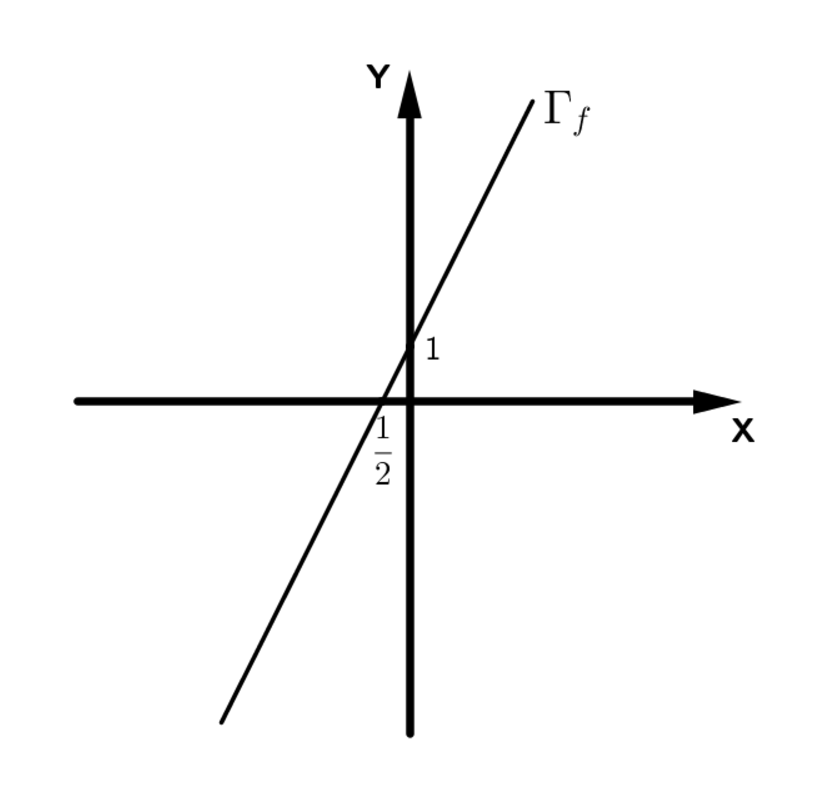
\includegraphics[scale=0.4]{sec1subgraphicotobr.eps}}
\end{figure}

\subsection{Вещественные  числа}
$\mathbb{R}$ -- множество вещественных чисел.

Аксиоматическое определение множества вещественных чисел:\\

{\bf \RomanNumeralCaps{1}.} в $\mathbb{R}$ введена операция сложения: $(x,y) \xrightarrow{\text{+}} z=x+y.$
\par Свойства действия сложения:
\begin{enumerate}
\item коммутативность \quad  $x+y=y+x,$ $\forall x, y ;$
\item ассоциативность \quad  $(x+y)+z=x+(y+z)=x+y+z,$ $\forall x, y, z ;$
\item существование нейтрального элемента (нуля) \quad $\forall x\;\;$ $x+0=x;$
\item существование противаположного элемента \quad $\forall x\;\;$  $\exists ! -x\;\;$ $x+(-x)=0.$
\end{enumerate}

{\bf \RomanNumeralCaps{2}.} В $\mathbb{R}$ введено умножение. $\cdot:(x,y)\rightarrow z=x\cdot y.$
\begin{enumerate}
\item коммутативность \quad $xy=yx;$
\item ассоциативность \quad $x(yz)=(xy)z=xyz;$
\item существование нейтрального элемента (единицы) \quad $1x=x;$
\item существование обратного элемента \quad $\forall x \; \exists x^{-1}: \; xx^{-1}=1.$
\end{enumerate}

{\bf \RomanNumeralCaps{3}.} Дистрибутивная связь. $(x+y)z=xz+yz.$

{\bf \RomanNumeralCaps{4}.} Отношение порядка. 

Некоторые пары $x,y\in\mathbb{R}$ удовлетворяют условию $x\leq y.$

Свойства отношения $\leq:$
\begin{enumerate}
\item рефлексивность \quad $x\leq x;$
\item антисимметричность \quad $x\leq y \& y\leq x \Rightarrow x=y;$
\item транзитивность \quad $x\leq y \& y\leq z \Rightarrow x\leq z.$
\end{enumerate}
-- общие свойства порядка.\\

{\bf \RomanNumeralCaps{5}.} Связь операций и порядка.

$x\leq y \Rightarrow x+z\leq x+z;$

$x\leq y \Rightarrow xz\leq yz.$
\newpage
{\bf \RomanNumeralCaps{6}.} Аксиома полноты.

Пусть $X, Y\subset \mathbb{R}$ и $\forall x\in X \; \forall y\in Y \; x\leq y.$ Тогда существует $c\in\mathbb{R}: \; \forall x\in X \; \forall y\in Y \; x\leq c\leq y.$
\begin{figure}[h]
\center{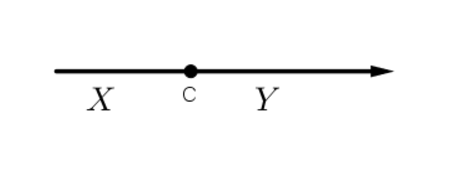
\includegraphics[scale=0.7]{sec1complitnessaxiom.eps}}
\end{figure}


\begin{Definition}
Пусть $E$ непустое подмножество вещественных чисел.

Число $M\in\mathbb{R}$ называется верхней границей $E,$ если $\forall x\in E\; x\leq M.$

Множество $E$ называется ограниченным сверху, если оно имеет верхнюю границу.

Число $m\in\mathbb{R}$ называется нижней границей $E,$ если $\forall x\in E\; m\leq x.$

Множество $E$ называется ограниченным снизу, если оно имеет нижнюю границу.

Наконец, множество $E$ называется ограниченным, если оно ограничено снизу и сверху: $\forall x\in E\; m\leq x\leq M.$
\end{Definition}

\begin{Theorem}
\begin{enumerate}
\item Если $E$ ограничено сверху, тогда среди верхних границ найдётся наименьшая.
\item Если $E$ ограничено снизу, тогда есть наибольшая нижняя граница.
\end{enumerate}
\end{Theorem}
\begin{proof}
\begin{enumerate}
\item Пусть $E$ ограничено сверху. За $E^s$ обозначим множество верхних границ $E.$ Тогда $\forall x\in E$ и $\forall y\in E^s \;\; x\leq y,$ значит, по аксиоме полноты $\exists c: \; \forall x\in E\; y\in E^s \quad x\leq c\leq y.$ При этом $c$ является верхней границей, так как $x\leq c$ и $c$ является наименьшей верхней границей, так как $c\leq y.$
\item Аналогично доказывается существование наибольшей нижней границы.
\end{enumerate}
\end{proof}

\begin{Definition}
\begin{enumerate}
\item Если $E$ ограничено сверху, тогда существует наименьшая верхняя граница, которая называется верхней гранью, точной верхней границей или супремумом и обозначается $\sup E$ или $\sup\limsup{x\in E}X.$
\item Если $E$ ограничено снизу, тогда существует наибольшая нижняя границы, которая называется нижней гранью, точной нижней границей или инфимумом и обозначается $\inf E$ или $\inf\liminf{x\in E}X.$
\end{enumerate}
\end{Definition}

\begin{Theorem}[Описание граней на $\varepsilon$-языке.]
Пусть $E$ непустое множество. 
\begin{enumerate}
\item $M=\sup E \Leftrightarrow \forall x\in E\; x\leq M$ и $\forall\varepsilon>0\; \exists x_0\in E: \; x_0>M-\varepsilon.$
\item $m=\inf E \Leftrightarrow \forall x\in E \; x\geq m$ и $\forall\varepsilon\; \exists x_0\in E: \; x_0<m+\varepsilon.$
\end{enumerate}
\end{Theorem}
\begin{proof}
$\Rightarrow:$\\
$m=\inf E, m$ -- нижняя граница: $\forall x\in E\; x\geq m.$ Значит $\forall\varepsilon>0\; m+\varepsilon>m$ и $m+\varepsilon$ -- не нижняя граница, то есть $\exists x_0\in E: \; x<m+\varepsilon.$\\
$\Leftarrow:$\\
$\forall x\in E$ и $x\geq m \;\; \forall\varepsilon>0\; \exists x\in E: \; x<m_\varepsilon.$ Тогда $m$ -- самая большая нижняя граница?
\par $\forall m'>m \; \varepsilon=m'-m>0 \; \exists x\in E$ (по условию), такой, что $x<m+\varepsilon = m+m'-m=m' \Rightarrow m'$ -- не нижняя граница, значит $m$ -- наибольшая нижняя граница (инфимум).
\end{proof}

\newpage
\par\medskip \textbf{Несколько предложений:}\par
\begin{enumerate}
\item $E_1\subset E$ -- ограничено сверху, тогда $E_1$ -- ограничено сверху и $\sup E_1\leq E$
\begin{proof}
$E$ -- ограничено сверху, значит $\exists M: \; \forall x\in E \; x<M \quad \forall x\in E_1 \; x\in E\; x\leq M$ то есть $E_1$ -- ограничено сверху.
\par $\forall x\in E_1\; x\in E \; x\leq \sup E \Rightarrow \sup E$ -- верхняя граница $E_1 \Rightarrow \sup E_1\leq \sup E.$
\end{proof}
\item $x_0\in\mathbb{R} \; E\subseteq\mathbb{R} \qquad E+x_0=\{x+x_0\mid x\in E\}$ -- сдвиг $E$ на $x_0.$
\par Если $E$ -- ограничено, то:
$$\sup\left(E+x_0\right)=\sup E+x_0$$
$$\inf\left(E+x_0\right)=\inf E+x_0$$
\item $\lambda\in\mathbb{R} \; E\subseteq\mathbb{R}, E\neq\varnothing \qquad \lambda E=\{\lambda x\mid x\in E\}.$
\par Если $E$ -- ограничено, то:
$$\sup\left(\lambda E\right)=\lambda\sup E$$
$$\inf\left(\lambda E\right)=\lambda\inf E$$
\end{enumerate}

\begin{Definition}
$x_0\in E$ называется наибольшим элементом множества $E,$ если $\forall x\in E\; x\leq x_0.$ Тогда $x_0=\max E.$
\end{Definition}

\par $x_0=\max E\Rightarrow x_0=\sup E$
\par $x_0=\sup E,\; x_0\in E \Rightarrow x=\max E,$ однако, если $x_0=\sup E$ и $x_0\notin E,$ то $x_0\neq\max E.$

\par\medskip \textbf{Несколько предложений:}\par
$\sup[0, 1] = \max[0, 1] = 1$
\par $\sup[0, 1) = 1 \neq \max[0, 1),$ так как $1\notin[0, 1).$ Более того, в $[0, 1)$ нет наибольшего элемента, так как если взять любое $M\in[0, 1),$ то $\frac{M+1}{2}\in[0, 1) \Rightarrow M$ не наибольший.
\subsection{Промежутки в множестве $\mathbb{R}$}
Промежуток есть множество одного из следующих типов:
\begin{enumerate}
\item $[a,b] =\{x\in\mathbb{R}\mid a\leq x\leq b\}$ -- отрезок
\item $(a,b) =\{x\in\mathbb{R}\mid a< x< b\}$ -- интервал
\item $[a,b) =\{x\in\mathbb{R}\mid a\leq x< b\}$ -- полуинтервал
\item $(a,b] =\{x\in\mathbb{R}\mid a< x\leq b\}$ -- полуинтервал
\item $[a, +\infty] =\{x\in\mathbb{R}\mid x\geq a\}$ -- луч
\item $[a,+\infty) =\{x\in\mathbb{R}\mid x>a\}$ -- луч
\item $[-\infty,b] =\{x\in\mathbb{R}\mid x\leq a\}$ -- луч
\item $[-\infty,b) =\{x\in\mathbb{R}\mid x<a\}$ -- луч
\item $[-\infty,+\infty) =\mathbb{R}$ 
\end{enumerate}

$\Delta\subseteq\mathbb{R}, \Delta\neq\varnothing$ -- промежуток $\Leftrightarrow \forall a, b\in\Delta\; \forall x \;\; a<x<b \Rightarrow x\in\Delta.$
\subsection{Геометрическая интерпретация}
$\mathbb{R}$ изображается прямой с отмеченными точками $0$ и $1.$
\begin{figure}[h]
\center{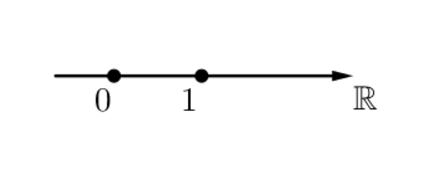
\includegraphics[scale=0.7]{sec1geominterpr.eps}}
\end{figure}
\subsection{Абсолютная величина вещественного числа}
\begin{Definition}
\begin{equation*}
\mid x\mid = 
 \begin{cases}
   x, & x>0\\
   0, & x=0\\
   -x, & x<0
 \end{cases}
\end{equation*}
\end{Definition}
\par\medskip \textbf{Свойства:}\par
\begin{enumerate}
\item $\mid x\mid \;=\max\{x;\; -x\}$
\item $\mid x\mid\;\leq 0 \qquad \mid x\mid\;=0 \Leftrightarrow x=0$
\item $\mid x\mid \;\;\mid -x\mid$
\item $\mid xy\mid\; =\;\mid x\mid\mid y\mid$
\item $\forall x\quad -\mid x\mid\leq x\leq\mid x\mid,$ действительно, $\mid x\mid=\max\{x;\; -x\} \;\; \mid x\mid\;\geq x\;\;\mid x\mid\;\geq -x\;\; x\geq-\mid x\mid$
\item $a>0 \;\; \mid x\mid\;\leq a \Rightarrow -a\leq x\leq a$\\
$\mid x\mid\;\leq a \Leftrightarrow \max\{x;\; -x\}\leq a \Leftrightarrow x\leq a \mathbin{\&} -x\leq a \Leftrightarrow x\leq a\mathbin{\&} x\geq -a \Leftrightarrow -a\leq x\leq a$
\item (неравенство треугольника) $\mid x+y\mid
\;\leq\;\mid x\mid+\mid y\mid$
\begin{proof}
$-\mid x\mid\leq x\leq\mid x\mid$\\
$-\mid y\mid\leq y\leq\mid y\mid$\\
$-(\mid x\mid+\mid y\mid)\leq x+y\leq\;\mid x\mid+\mid y\mid,$ по свойству $6,$ обозначив за $a=\;\mid x\mid+\mid y\mid,$ получим $\mid x+y\mid\;\leq\;\mid x\mid+\mid y\mid.$
\end{proof}
\item $\mid x-y\mid\;\leq\;\mid x\mid+\mid y\mid$
\item $\mid x-y\mid\;\leq\;\mid\mid x\mid-\mid y\mid\mid$
\begin{proof}
$\mid x\mid\;=\;\mid(x-y)+y\mid\;\leq\;\mid x-y\mid+\mid y\mid \qquad \mid x\mid-\mid y\mid\;\leq\;\mid x-y\mid.$\\
Аналогично $\mid y\mid-\mid x\mid\;\leq\;\mid x-y\mid,$ таким образом $\max\{\mid x\mid+\mid y\mid, \mid y\mid=\mid x\mid\}\leq\l\mid x+y\mid,$ отсюда $\mid\mid x\mid -\mid y\mid\mid\;leq\;\mid x-y\mid.$
\end{proof}
\item $\mid x+y\mid\; \leq\;\mid\mid x\mid-\mid y\mid\mid$
\end{enumerate}

\begin{Proposition}
Пусть $E\subset\mathbb{R}, \; E$ ограничено $\Leftrightarrow \; \exists M: \; \forall x\in E \; \mid x\mid\;\leq M.$
\end{Proposition}
\begin{proof}
$\Rightarrow:$\\
Так как $E$ ограничено, то $\exists m, M: \; \forall x\in E \; m\leq x\leq M.$ Обозначим за $M_1=\max\{\mid m\mid;\;\mid M\mid\}.$ Теперь $\forall x\in E \; \mid x\mid\;\leq M_1,$ таким образом $\forall x\in E \; m\leq x<M\leq\;\mid M\mid\;\leq M_1$ и $-x\leq-m\leq\;\mid m\mid\;\leq M_1.$ \\
$\Leftarrow:$\\
$\forall x \; \mid x\mid\;\leq M, \;\; -M\leq x\leq M$ откуда сразу следует ограниченность $E.$
\end{proof}
\subsection{Натуральные числа}
\begin{Definition}
Множество $E\in\mathbb{R}$ называется индуктивным, если $\forall x\in E \; x+1\in E.$

$\mathbb{N}$ -- наименьшее индуктивное множество, содержащее $1\in\mathbb{N},$ тогда $\mathbb{N}$ называется натуральным рядом, а элементы этого множества -- натуральными числами.

$\mathbb{N}=\bigcap\limits_{1\in E}E, \; E$ -- индуктивно. 
\end{Definition}

\par\medskip \textbf{Примеры индуктивных множеств}\par
$\mathbb{R};$

$[1, +\infty).$

\subsubsection{Принцип математической индукции}
Пусть $E$ подмножество натуральных чисел $E\subset\mathbb{N}$ и $1\in E.$ Тогда, если $\forall n\in E$\\ $n+1\in E,$ то $E=\mathbb{N}.$

Доказательства методом математической индукции:
\begin{enumerate}
\item База: $n=1\in\mathbb{N};$
\item Переход: если утверждение справедливо для некого $n,$ то оно справедливо и для $n+1,$ тогда $\forall n$ утверждение выполнено.
\end{enumerate}

\begin{Proposition}
Неравенство между средним арифметическим и средним геометрическим.

$a_1, a_2,\ldots, a_n\in\mathbb{R} \;\;\; \frac{a_1+a_2+\ldots+a_n}{n}$
\smallskip
\par $\forall i \; a_i>0 \;\;\; \sqrt[n]{a_1\cdot a_2\cdot\cdots\cdot a_n}$

\smallskip
Тогда $\sqrt[n]{a_1\cdot a_2\cdot\cdots\cdot a_n}\leq\frac{a_1+a_2+\ldots+a_n}{n},$ причём равенство достигается только при $a_1=a_2=\ldots=a_n.$
\end{Proposition}

\begin{Proposition}
$a_1,\ldots, a_n>0,$ тогда $a_1+\ldots+a_n\geq n$ и равенство достигается только при $a_1=\ldots=a_n=1.$
\end{Proposition}
\begin{proof}
Если $a_1=\ldots=a_n=1$ -- очевидно.

Пусть не все числа равны $1.$ Будем считать, что $a_{n-1}<1, a_n>1.$
\begin{enumerate}
\item База: $n=2\;$ $(1-a_1)(a_2-1)>0,\;$ $a_1+a_2-1-a_1a_2>0,\;$ $a_1+a_2-2>0,\;$ $a_1+a_2-2>0,\;$ $a_1+a_2>2$ что и требовалось доказать.
\item Переход: пусть для $n$ чисел неравенство выполнено. 

$a_1,\ldots, a_n, a_{n+1}>0\;$ $a_n<1 \; a_{n+1}>1.$ Применим индукцию:

$a_1+\ldots+a_{n-1}+a_n\cdot a_{n+1}\geq n,\;$ $(1-a_n)(a_{n+1}-1)>),\;$ $a_n+a_{n+1}-a_na_{n+1}>1,\;$ $a_1+\ldots+a_{n+1}>n+1.$  
\end{enumerate}
\end{proof}

Теперь докажем предложение $2:$
\begin{proof}
$a_1,\ldots, a_n>0.$ Обозначим $A=\sqrt[n]{a_1\cdot a_2\cdot\cdots\cdot a_n}$ и $b_k=\frac{a_k}{A}, k=1,..,n.$ 

Легко заметить, что $b_1\cdot b_2\cdot\ldots\cdot b_n\cdot\frac{a_1\cdot\ldots\cdot a_n}{A^n}=1.$

Как видно, $b_1,\ldots, b_n$ -- удовлетворяют условию предложения $2,$ тогда $b_1+\ldots+b_n\geq n, \;\; a_1+\ldots+a_n\geq nA$
\par $\frac{a_1+a_2+\ldots+a_n}{n}\geq\sqrt[n]{a_1\cdot a_2\cdot\cdots\cdot a_n}$
\end{proof}

\par\medskip \textbf{Свойства множества $\mathbb{N}:$}\par
\begin{enumerate}
\item В $\mathbb{N}$ выполнимы операции $"+", "\cdot": \;\; \forall n, m\in\mathbb{N} \; n+m\in\mathbb{N}, \; n\cdot m\in\mathbb{N};$
\item $1=\min\mathbb{N},$ действительно $1\in[1, +\infty)$ -- индуктивно, значит $\mathbb{N}\subset[1, +\infty)\;\; \forall n\in\mathbb{N} \; n\leq1;$
\item $\forall n\in\mathbb{N}\;\; n\neq 1 \Rightarrow n-1\in\mathbb{N};$
\item $\forall n\in\mathbb{R} \; \mathbb{N}\cap (n, n=1)=\varnothing;$
\item $E\subseteq\mathbb{R} \Rightarrow E$ ограничено снизу, тогда $E$ имеет наименьший элемент.
\item $E\subseteq\mathbb{R} \Rightarrow E$ ограничено сверху, тогда $E$ имеет наибольший элемент.
\item Принцип Архимеда.
\par $\forall\varepsilon>0\; \varepsilon\mathbb{N}$ не ограничено сверху. В частности $\mathbb{N}$ не ограниченное сверху множество. 

$\varepsilon\mathbb{N}=\{\varepsilon n\mid n\in\mathbb{N}\}=\{\varepsilon, 2\varepsilon, 3\varepsilon,\ldots\}$
\begin{proof}
Пусть $\varepsilon\mathbb{N}$ ограничено сверху, тогда $M=\sup\varepsilon\mathbb{N},$ но обязательно будет существовать $n\in\mathbb{N}: \; n\varepsilon>M\varepsilon,$ если нет, то $(1+n)\varepsilon>M.$ Значит есть $k=n+1\in\mathbb{N}: \; k\varepsilon>M$ -- противоречие
\end{proof}

\begin{Corollary}
$\forall\varepsilon>0 \; \exists n\in\mathbb{N}: \;\; \frac{1}{n}<\varepsilon \qquad \left(\frac{1}{n}<\varepsilon \Leftrightarrow n\varepsilon>1\right).$
\end{Corollary}

\begin{Corollary}
$\forall n \; 0\leq x<\frac{1}{n} \Rightarrow x=0.$
\end{Corollary}
\end{enumerate}

\subsection{Целые числа}
\begin{Definition}
Множество целых чисел $\mathbb{Z}=\mathbb{N}\cup\{0\}\cup\{-\mathbb{N}\}.$
\end{Definition}

\par\medskip \textbf{Свойства $\mathbb{Z}:$}\par
\begin{enumerate}
\item $\forall m, n\in \mathbb{Z}$ определены $m+n, m-n, m\cdot n \in\mathbb{Z};$
\item $\forall n\in\mathbb{Z}\;\; \mathbb{Z}\cap(n, n+1)=\varnothing;$
\item Всякое ограниченное сверху множество целых чисел имеет наибольший элемент.
\par Всякое ограниченное снизу множество целых чисел имеет наименьший элемент.
\begin{proof}
Пусть $E\subset\mathbb{Z}, E$ -- ограничено сверху и $M=\sup E.$ Тогда $\exists n\in E \; n>M-1 \;\; n =\max E.$ Если найдётся $m\in E$ такой, что $m>n, n\leq m\leq n+1,$ то получится, что $n\in(n, n+1)$ -- противоречие, значит $n$ действительно наибольший элемент $E.$

Аналогично доказывается про наименьший элемент.
\end{proof}
\item Пусть $\rho>0, x\in\mathbb{R},$ по принципу Архимеда $\exists m\in\mathbb{Z}: \; m\rho>x.$ Такие $x$ образуют ограниченное снизу множество. Выберем наименьшее $m:\;\; m\rho>x \mathbin{\&} (m-1)\rho\leq x.$ Примем $n=m-1,$ тогда $n\rho\leq x< (n+1)\rho.$ Выходит, что $x\in[n\rho, (n+1)\rho).$ 

Таким образом $\mathbb{R}$ разбилось на непересекающиеся промежутки $[n\rho, (n+1)\rho)], n\in\mathbb{Z}.$

При $\rho=1 \; \forall x\in\mathbb{R} \; \exists! n: \; x\in[n,n+1),$ тогда $n=[x]$ называется целой частью $x$ или антье $x,$ $\{x\}=x-[x]$ называется дробной частью $x.$
\end{enumerate}
\subsection{Рациональные числа}

\begin{Definition}
Множество рациональных чисел обозначается как $\mathbb{Q}$ и состоит из элементов вида $\frac{m}{n},$ где $n\in \mathbb{N}$ и $m\in\mathbb{Z}.$
\end{Definition}

\begin{Definition}
Множество $X$ называется плотным во множестве $Y$ \quad $\Leftrightarrow$ \quad $\Leftrightarrow$ $\forall \alpha, \beta \in \mathbb{Y}:$ $\alpha<\beta \quad \exists x\in X: x\in(\alpha,\beta.)$
\end{Definition}

\begin{Theorem}
$\mathbb{Q}$ плотно в $\mathbb{R}.$
\end{Theorem}
\begin{proof}
Возьмём $\varepsilon = \beta - \alpha > 0.$ По принципу Архимеда $\exists n\in \mathbb{N}: \; \frac{1}{n}<\varepsilon$ и $\exists m\in\mathbb{Z}: \; \frac{m}{n} >\alpha.$ Среди таких чисел выберем наименьшее $m$ такое, что $\frac{m}{n}>\alpha,$ тогда $\frac{m-1}{n}\leq \alpha.$ Обозначая $x=\frac{m}{n}$ получаем, что $X\in(\alpha,\beta).$ Ну, действительно, известно, что $\frac{m-1}{n}<\alpha,$ тогда $\frac{m}{n}\leq\alpha+\frac{1}{n},$ то есть $x\leq \alpha+
\frac{1}{n}<\alpha+\varepsilon=\beta,$ откуда $\alpha < \beta.$
\end{proof}

\begin{Proposition}
Любое вещественное число можно с любой степенью точности приблизить рациональными числами. 
\end{Proposition}
\begin{proof}
Возьмём $x\in(0,1].$ Среди десятичных дробей: $0.1, 0.2,\ldots, 0.9$ выберем наибольшую из тех, что меньше $x.$ Пусть эта дробь равна $0.\alpha_1.$ Теперь возьмём $x_1$ -- меньшее $x,$ но $x_1+\frac{1}{10}>x.$
\smallskip

Среди дробей: $0.\alpha_1 1, 0.\alpha_1 2,\ldots, 0.\alpha_1 9$ выберем $x_2=0.\alpha_1\alpha_2: x_2<x<x_2+\frac{1}{100}.$ 
\smallskip

Таким образом получаем последовательность десятичных дробей $x_n=0.\alpha_1\alpha_2\ldots\alpha_n: x_n<x<x_n+\frac{1}{10^n}.$ Тогда бесконечная дробь $x=0.\alpha_1\alpha_2\ldots\alpha_n\ldots$ представляет вещественное число $x.$
\end{proof}

В $\mathbb{Q}$ выполнены все арифетические действия.
\subsection{Мощность}
\begin{Definition}
Множества $X$ и $Y$ равномощны, если $\exists f:X\rightarrow Y$ -- инъективное отображение. Записывается как $X\sim Y; \mid X\mid=\mid Y\mid$ или как $cardX=cardY.$ (\textit{кардинальное число $X$})
\end{Definition}

Заметим, что если $X\subseteq Y,$ то $\mid X\mid \leq\mid Y\mid.$\\

\begin{Proposition}
Множество натуральных чисел $\mathbb{N}$ равномощно множеству чётных чисел $\mathbb{N}_{2n}.$
\end{Proposition}
\begin{proof}
Ну, действительно, возьмём функцию $f(n)=2n.$ Легко понять, что $f$ биекция, значит, по определению, множества равномощны.
\end{proof}

\begin{Theorem}[Шредер-Бернштейн]
Если $\mid X\mid\leq\mid Y\mid$ и $\mid Y\mid\leq X\mid,$ то $\mid X\mid = \mid Y\mid.$
\end{Theorem} 

Любые два множества сравнимы по мощности: $\mid X\mid<\mid Y\mid\vee \mid X\mid=\mid Y\mid\vee \mid X\mid>\mid Y\mid.$ 

\begin{Theorem}[Кантора]
Пусть $X$ -- множество, $\mathcal{P}(X)$ -- множество всех подмножеств $X.$ Тогда $\mid\mathcal{P}(X)\mid >\mid X\mid.$
\end{Theorem}
\begin{proof}
Рассмотрим отображение $X\rightarrow\mathcal{P}(X)$ такое, что $x\in X \rightarrow\{x\}\in\mathcal{P}(X)$ -- инъекция, значит $\mathcal{P}(X)\mid\geq\mid X\mid.$ Теперь покажем, что $\mid \mathbb{P}(X)\mid \neq\mid X\mid:$\\

Предположим, что $\mathcal{P}(X)\mid=\mid X\mid,$ тогда $f:X \rightarrow \mathcal{P}(X)$ -- сюръекция, тогда $\forall y \in Y \; Y=f(y)\in\mathcal{P}(X), Y\subseteq X.$ Рассмотрим $Y_0=\{y\in X\mid y\notin f(y)\},$  $Y_0\subseteq X,$ значит $Y_0\in\mathcal{P}(X).$ Так как $f$ сюръекция, то $\exists y_0 \in Y_0: \; f(y_0)=Y_0.$\\

Будет ли верно, что $y_0\in Y_0?$ Ну, проверим: пусть $y_0\in Y_0,$ следовательно $y_0 \neq f(y_0)=Y$ -- противоречие, значит $y_0 \notin Y_0,$ но $Y_0 = f(y_0),$ откуда $y_0\in Y_0$ -- противоречие, значит $f$ не сюръекция.
\end{proof}
\smallskip
\smallskip
\subsubsection{Конечное множество}
Пусть $n\in\mathbb{N},$ тогда $\mathbb{N}_n=\{m\in\mathbb{N}\mid m\leq n\}=\{1, 2,\ldots, n\}$ -- отрезок натурального ряда.
\begin{Definition}
Если $X\sim \mathbb{N}_n,$ то $X$ называется конечным множеством и $n=card X$ -- число элементов $X.$
\end{Definition}

Если $n\neq m,$ то $\mid\mathbb{N}_n\neq\mathbb{N}_m.$

\begin{Proposition}
Множество $X$ конечно $\Leftrightarrow$ $X$ не равномощно своей правильной части$.$ $\mid X\mid\neq\mid Y\mid$, при $Y\subseteq X$ и $Y\neq Y.$
\end{Proposition}

Рассмотрим отображение из $\mathbb{N}$ в $\mathbb{N}\setminus\{1\}$ такое, что $n \rightarrow n+1.$ Так как отображение биективно, то множество $\mathbb{N}\setminus\{1\}$ не конечно.
\begin{Definition}
Бесконечное множество -- не конечное множество.
\end{Definition}

\subsubsection{Счётное множество}
Пусть $X$ бесконечное множество, тогда, если $\forall n \; \exists x_1,\ldots, x_n \in X$ -- попарно различны, то $\exists x_1,\ldots, x_n, x_{n+1} \in X$ -- попарно различны.\\

Тогда $x_1,\ldots$ образуют множество, равновощное множеству натуральных чисел. Таким образом $\mathbb{N}$ самое маленькое бесконечное множество.

\begin{Definition}
Если множество $X$ счётно, то пишут, что его мощность $cardX=\aleph_0$ (\textit{Алеф ноль})$.$
\end{Definition}

Если множество $X$ конечно или счётно, то $X$ называется не более чем счётным множеством.

Пусть $X$ счётно, тогда $\mathcal{X}$ несчётно.\\

\begin{Proposition}
$\mathbb{Z}$ -- счётно.
\end{Proposition}
\begin{proof}
Определим биективное отображение из $\mathbb{N}$ в $\mathbb{Z}$ следующим образом: 
\begin{equation*}
f(x) = 
 \begin{cases}
   \frac{n}{2}, &\text{ $n = 0(mod \; 2) $}\\
   \frac{n-1}{2}, &\text{ $n = 1(mod \; 2)$}
 \end{cases}
\end{equation*}
\end{proof}

\begin{Proposition}
$\mathbb{N^2}\sim\mathbb{N}$ 
\end{Proposition}
\begin{proof}
Ну, действительно, запишем сначала все пары натуральных чисел с первым элементом равным $1$, ниже все пары, начинающиеся с $2$ и так далее. Начнём нумеровать пары следующим образом:
$$(1,1) - 1 \;\; (1,2) - 2 \;\; (1,3) - 6 \ldots$$
$$(2,1) - 3 \;\; (2,2) - 5 \;\; (2,3) - 7 \ldots$$
$$(3,1) - 4 \;\; (3,2) - 8 \;\; (3,3) - 12 \ldots$$
$$\vdots \quad\quad\quad\quad\vdots \quad\quad\quad\quad\vdots$$
Так как каждый раз диагонали будут конечными, то удастся занумеровать все пары.
\end{proof}

\begin{Proposition}
$\mathbb{Q}$ счётно.
\end{Proposition}
\begin{proof}
Очевидно, что $\mid\mathbb{Q}\mid \geq\mid\mathbb{N}\mid.$ Докажем равенство.\\
Докажем, что $\mid\mathbb{Q}\mid \leq\mid\mathbb{N}\mid:$ \\
Любое $x\in\mathbb{Q}$ представляется в виде несократимой дроби $\frac{m}{n}, \; m\in\mathbb{Z}, \; n\in\mathbb{N}.$ Тогда запишем $card\mathbb{Q}\leq card\mathbb{Z}\times\mathbb{N} = card\mathbb{N}\times\mathbb{N}=card\mathbb{N}.$\\
Отсюда имеем, что $\mid\mathbb{Q}\mid \geq\mid\mathbb{N}\mid$ и $\mid\mathbb{Q}\mid \leq\mid\mathbb{N}\mid,$ следовательно $\mid\mathbb{Q}\mid =\mid\mathbb{N}\mid$
\end{proof}

\subsubsection{Мощность континуум}
\begin{Proposition}
Множество вещественных чисел $\mathbb{R}$ и $\mathcal{P}(\mathbb{N})$ равномощны.
\end{Proposition}
\begin{proof}
\begin{enumerate}
\item $x\in\mathbb{R} \longmapsto (-\infty, x)\cap\mathbb{Q} \subset \mathbb{Q}.$ Тем самым определено инъективное отображение множества $\mathbb{R} \rightarrow\mathcal{P}(\mathbb{Q}),$ поэтому $card\mathbb{R}\leq card\mathcal{P}(\mathbb{Q})=card\mathbb{N}.$
\item Рассмотрим некое подмножество натуральных чисел $A\subset\mathbb{N}.$ Построим бесконечные десятичные дроби $x=0.\alpha_1\alpha_2\cdots$ по следующему правилу:
\begin{equation*}
\alpha_n = 
 \begin{cases}
   1, &\text{ $n\in A $}\\
   0, &\text{ $n\notin A$}
 \end{cases}
\end{equation*}
Таким образом определена индукция $\mathcal{P}(\mathbb{N}) \rightarrow [0, 1),$ 
\end{enumerate} 
значит $$card\mathcal{P}(\mathbb{N})\leq card\mathbb{R} \Rightarrow card\mathbb{R}= card\mathcal{P}(\mathbb{N}).$$
\end{proof}

\begin{Definition}
Если $X\sim\mathcal{P}(\mathbb{N})\sim\mathbb{R},$ то говорят, что $x$ имеет мощность континуум и обозначают $cardX=c=2^{\aleph_0}.$
\end{Definition}

\newpage

\section{\LARGE{\bf Предел функции}}
\newpage

\begin{center}
\section{\LARGE{\bf Предел функции}}
\end{center}
\epigraph{\textit{Ну а это вы изучите сами дома.}}
{-- Моисеев А.А.}
\subsection{Понятие предела функции}
\subparagraph{Предельная точка}
\begin{Definition}
Пусть $E\subseteq\mathbb{R}$ и $a\in\mathbb{R}.$ $a$ называется предельной точкой для $E,$ если $\forall\delta> 0\;\exists x\in E: \; 0<\mid x-a\mid<\delta.$
\end{Definition}

Рассмотрим множество на числовой прямой $(a, b)\cup\{c\}.$ Точки $a$ и $b$ -- предельные точки множества. Точка $c$ называется изолированной точкой множества.



$a$ предельная, если $\forall O$ окрестности $a \; \exists x\in O\cap E, x \neq a.$

Помимо обычной окрестности точки вводят также определение проколотой окрестности: $\dot{O} = O\setminus\{a\}.$

Таким образом, $a$ предельная точка для $E,$ если $\forall O$ -- окрестности точки $a$ выполнено, что $E\cap\dot{O}\neq\varnothing.$

\subparagraph{Определение предела функции}

\begin{Definition}
$E\subseteq\mathbb{R}, a$ -- предельная точка $E, \; f$ -- функция на $\mathbb{E}, A\in\mathbb{R}. \; A$ называется пределом функции $f$ в точке $a, \;f(x)\xrightarrow[x\rightarrow a]{} A; \; A=\lim\limits_{x\rightarrow a} f(x); A=\lim\limits_{a}f,$ если:
\begin{enumerate}
\item на языке $\varepsilon$-$\delta:$

$\forall \varepsilon > 0 \;\exists \delta > 0\;\forall x\in E 0<\mid x-a\mid<\delta \Rightarrow \mid f(x)-A\mid<\varepsilon;$

\item на языке окреcтностей$:$

$\forall O$ окрестности точки $A$ $\exists V$ -- окрестность точки $a: \; f(\dot{V}\cap E \subset O;$

\item на языке последовательностей$:$

$\forall\{x_n\} \; x_n\in E \; x_n \neq a, \; x_n\xrightarrow[n \rightarrow \infty]{} a,  \Rightarrow f(x_n)\xrightarrow[n\rightarrow\infty]{} A.$
\end{enumerate}
\end{Definition}

\par\medskip \textbf{Пример}\par

%КАРТИНКА!!!!!!!!!!!!!!!!!!!!!!!!!!!!!!!!!!!!!!!!!!!!!!!!!!!!!!!!!!!!!!!!!!!!!!!!

Предел -- локальное понятие. Если $f=g$ в $\dot{O}$ проколотой окрестности точки $a,$ то они имеют пределы и они равны.

\subparagraph{Равносильность определений}
\begin{Theorem}[Равносильность определений]
Определения (1), (2) и (3) равносильны. Если $A=\lim\limits_{x \to a} f(x)$ в смысле одного из определений, то $A=\lim\limits_{x \to a} f(x)$ и в смысле других определений.
\end{Theorem}
\begin{proof}
Для начала сравним определения (1) и (2).
Пусть $A=\lim\limits_{x \to a} f(x)$ в смысле (1). Возьмём произвольную окрестность $V$ точки $A$. Найдётся такое $\varepsilon>0$, что $V_\varepsilon(A) \subset V$. По определению (1) существует такое $\delta > 0$, что
$$x \in E, x \neq a, \; \mid x - a \mid \; < \varepsilon \Rightarrow \mid f(x) - A \mid \; < \varepsilon.$$
Полагая $U = V_\delta (a)$, можно переписать предыдущее соотношение в виде $f(U \cap E) \in V_\varepsilon(A) \in V$. Таким образом, $A=\lim\limits_{x \to a} f(x)$ в смысле (2).
Наоборот, пусть $A=\lim\limits_{x \to a} f(x)$ в смысле (2). Возьмём произвольное $\varepsilon > 0$ и положим $V = V_\varepsilon(A)$. По определению (2) найдётся окрестность $U$ точки $a$, для которой $f(U \cap E) \in V$. Подберём $\delta > 0$, для которого $V_\delta(a) \in U$. Теперь
$$\forall x \in E, 0 < \; \mid x - a \mid \; < \delta \Rightarrow \mid f(x) - A \mid<\varepsilon,$$
$A=\lim\limits_{x \to a} f(x)$ в смысле (2). Установлена равносильность определений (1), (2).
Докажем равносильность определений (1), (3).
Пусть $A=\lim\limits_{x \to a} f(x)$ в смысле (1). Возьмём произвольную последовательность
$${x_n}, x_n \neq a, x_n \xrightarrow[n\rightarrow\infty]{} a.$$
и убедимся в том, что $f(x_n) \xrightarrow[n\rightarrow\infty]{} A.$
Возьмём произвольное $\varepsilon > 0$. По определению (1) найдётся такое $\delta > 0$, что
$$\forall x \in E, 0 < \; \mid x - a \mid \; < \delta \Rightarrow \mid f(x) - A \mid < \varepsilon.$$
По определению предела последовательности найдётся номер $N$, для которого
$$ n > N \Rightarrow \mid x_n - a \mid \; < \delta.$$
Видим, что при $n > N$ выполняется соотношение $\mid f(x_n) - A \mid \;  < \varepsilon.$ Итак, $f(x_n) \xrightarrow[n\rightarrow\infty]{} A.$ $A=\lim\limits_{x \to a} f(x)$ в смысле (3).
Пусть $A=\lim\limits_{x \to a} f(x)$ в смысле (3). Допустим, $A$ не является пределом в смысле (1). Тогда
$$\exists\varepsilon > 0 \; \forall \delta > 0 \; \exists x \in E, 0 < \;  \mid x - a \mid \; < \delta, \; \mid f(x) - A \mid \; \geq \varepsilon.$$
В качестве $\delta > 0 $ последовательно возьмём числа $\frac1{n}$, $n = 1, 2, \ldots$ и найдём точки $x_n \in E, 0 < \; \mid x_n - a \mid \; < \frac1{n}, \; \mid f(x_n) - A \mid \; \geq \varepsilon$. Тем самым мы получаем последовательность ${x_n}$. Неравенство $\mid x_n - a \mid < \frac1{n} $ означает, что $x_n \xrightarrow[n\rightarrow\infty]{} a$, а неравенство $\mid f(x_n) - A \mid \geq \varepsilon$ говорит, что $A$ не является пределом для ${f(x_n)}$, вопреки предположению. Полученное противоречие заставляет нас признать, что $A=\lim\limits_{x \to a} f(x)$ в смысле (1).
\end{proof}
\subsection{Различные предельные конструкции}
\subparagraph{Односторонние пределы}
Пусть $f$ определена на некотором интервале $(a - \delta_0, a)$.
Число $A$ -- левосторонний предел функции $f$ в точке $a$ $(A = f(a - 0)$, $A=\lim\limits_{x \to a - 0} f(x), f(x) \xrightarrow[n\rightarrow a-0]{} A),$ если
$$ \forall \varepsilon > 0 \; \exists \delta > 0 \; \forall x: a - \delta < x < a \Rightarrow \; \mid f(x) - A \mid \; < \varepsilon.$$
Пусть $f$ определена на некотором интервале $(a, a + \delta_0)$.
Число $A$ называется правосторонним пределом функции $f$ в точке $a (a = f(a+0), A=\lim\limits_{x \to a+0} f(x)), f(x) \xrightarrow[n\rightarrow a+0]{} A),$ если
$$ \forall \varepsilon > 0 \; \exists \delta > 0 \; \forall x: a < x < a + \delta \Rightarrow \; \mid f(x) - A \mid \; < \varepsilon.$$
Определения односторонних пределов можно дать и в терминах окрестностей и последовательностей.
\begin{Proposition}
Функция $f$ определена в проколотой окрестности точки $a$.
Тогда функция имеет предел в точке $a$ в том и только том случае, если существуют и равны между собой односторонние пределы $f(a-0) = f(a+0).$ В случае существования предела
$$f(a-0) = f(a+0) = \lim\limits_{x \to a} f(x)$$
\end{Proposition}

\subparagraph{Бесконечные пределы}
В определении предела число $A$ можно заменить на $+\infty$, $-\infty$, $\infty$. Например,
$$f(x) \xrightarrow[x\rightarrow a]{} -\infty \Leftrightarrow \forall E > 0 \; \exists \delta > 0, \; 0 < \; \mid x - a \mid \; < \delta \Rightarrow f(x) < -E.$$

\subparagraph{Пределы на бесконечности}
Бесконечности могут выполнять и роль точки, в которой вычисляется предел. Например,
$$f(x) \xrightarrow[x\rightarrow a]{} \infty \Leftrightarrow \forall E > 0 \; \exists \delta > 0: x > \delta \Rightarrow \; \mid f(x) \mid \; > E.$$

\subsection{Простейшие свойства предела функции}
\begin{enumerate}
\item Если функция постоянна в некотрой проколотой окрестности точки $a$, $f(x) = A$ при $x \in V$, то $f(x) \xrightarrow[x\rightarrow a]{} A.$
\item Предел единственен.
\item Если функция имеет конечный предел, то она она ограничена в некотрой проколотой окрестности.
\end{enumerate}

\subsection{Предел и арифметические операции}
\begin{Theorem}
Пусть функции $f, g$ определены в проколотой окрестности $E$ точки $a$.
$$f(x) \xrightarrow[x\rightarrow a]{} A, g(x) \xrightarrow[x\rightarrow a]{} B.$$
Определим функции
$$F: F(x) = f(x) + g(x), x \in E;$$
$$G: G(x) = f(x) \cdot g(x), x \in E;$$
$$H: H(x) = \frac{f(x)}{g(x)}, x \in E.$$
(В последнем случае предполагаем, что $g(x) \neq 0$ при $x \in E$).
Тогда функции $F, G, H$ тоже имеют пределы,
$$F(x) \xrightarrow[x\rightarrow a]{} A + B, G(x) \xrightarrow[x\rightarrow a]{} A \cdot B, H(x) \xrightarrow[x\rightarrow a]{} \frac{A}{B}$$
(последнее при условии $B \neq 0$).
\end{Theorem}

\begin{proof}
Докажем, например, последнее утверждение.
Возьмём произвольную последовательность ${x_n}, x_n \in E, x_n \neq a, x_n \xrightarrow[n\rightarrow \infty]{} B.$
По теореме о пределе отношения последовательностей $H(x_n) \xrightarrow[n \rightarrow \infty]{} \frac{A}{B}.$ Опять по определению предела функции $H(x) \xrightarrow[x \rightarrow a]{} \frac{A}{B}.$
\end{proof}

\subsection{Предел и неравенства}
\begin{Theorem}
Пусть функции $f, g$ определены в проколотой окрестности $E$ точки $a$.

\subparagraph{Стабилизация неравенств}
$$f(x) \xrightarrow[x \rightarrow a]{} A, g(x) \xrightarrow[x \rightarrow a]{} B, A < B.$$
Тогда
$$\exists U \; \forall x \in U, f(x) < g(x).$$

\subparagraph{Предельный переход в неравенстве}
$$\forall x \in E, f(x) < g(x),$$
$$f(x) \xrightarrow[x \rightarrow a]{} A, g(x) \xrightarrow[x \rightarrow a]{} B,$$
Тогда
$$A \leq B.$$
\begin{Remark}
Можно ослабить условие и потребовать выполнения неравенства $f(x) \leq g(x)$ в некоторой проколотой окрестности точки $a$.
\end{Remark}

\subparagraph{Теорема о полицейских}
$$\forall x \in E, f(x) \leq h(x) \leq g(x),$$
$$f(x) \xrightarrow[x \rightarrow a]{} A, g(x) \xrightarrow[x \rightarrow a]{} A.$$
Тогда
$$h(x) \xrightarrow[x \rightarrow a]{} A.$$

\end{Theorem}
\begin{proof}
Рассмотрим окрестности $V_A = \left( -\infty;\frac{A+B}{2} \right)$ и $V_B = \left(\frac{A+B}{2};+\infty \right)$ точек $A$ и $B$ соответственно. На основании определения предела мы можем найти такую окрестность $U$ точки $a$, что при $x \in U$ справедливы включения $f(x) \in V_A$ и $g(x) \in V_B$. $U$ -- искомая окрестность. Поскольку из $f(x) \in V_A$ следует, что $f(x) < \frac{A+B}{2}$, а $g(x) \in V_B$ влечёт $g(x) > \frac{A+B}{2}$, то $f(x) < g(x)$.

Утверждение о предельном переходе в неравенстве доказывается, как и в случае последовательностей, методом от противного. Допустив, что имеет место неравенство $A > B$, мы придём к противоречащему условию выводу о том, что в пределах некоторой проколотой окрестности точки $a$ выполняется неравенство $f(x) > g(x)$.

Возьмём произвольную последовательность ${x_n}, x_n \neq a, x_n \xrightarrow[n \rightarrow \infty]{} a.$

По определению предела на языке последовательностей получаем соотношения $f(x_n) \xrightarrow[n \rightarrow \infty]{} A, g(x_n) \xrightarrow[n \rightarrow \infty]{} A$, а по условию $f(x_n) \leq h(x_n) \leq g(x_n), n = 1, 2, \ldots$ По теореме о полицейских для последовательностей $h(x_n) \xrightarrow[n \rightarrow \infty]{} A$. Вновь пользуясь определением на языке последовательностей, делаем вывод, что $h(x_n) \xrightarrow[n \rightarrow \infty]{} A$.
\end{proof}

\subsection{Бесконечно малые и бесконечно большие функции}
\subparagraph{Бесконечно малые функции}
\begin{Definition}
Функция $\alpha$ -- бесконечно малая при $x \rightarrow a$, если $\alpha(x) \xrightarrow[x \rightarrow a]{} 0$.
\end{Definition}
\begin{Theorem}Сумма бесконечно малых является бесконечно малой.\end{Theorem}
\begin{Theorem}Произведение бесконечно малой на ограниченную функцию является бесконечно малой. \end{Theorem}
\begin{Theorem}[Определение предела в терминах бесконечно малых]
$$f(x) \xrightarrow[x \rightarrow a]{} A \Leftrightarrow \alpha = f - A -- б. м.$$
\end{Theorem}
\subparagraph{Бесконечно большие функции}
\begin{Definition}Функция $f$ называется бесконечно большой ($f(x) \xrightarrow[x \rightarrow a]{} \infty)$, если
$$\forall E > 0 \; \exists \delta > 0, \; 0 < \; \mid x - a \mid \; < \delta \Leftrightarrow \; \mid f(x) \mid \; > E.$$
\end{Definition}

\begin{Theorem} $\alpha$ -- б. м. $\Leftrightarrow f = \frac{1}{\alpha}$ -- б. б. \end{Theorem}

\subsection{Предел монотонной функции}
\begin{Definition}
Пусть $f$ -- функция, определённая на промежутке $\Delta$.
\end{Definition}

\begin{itemize}
\item Функция $f$ называется возрастающей (строго возрастающей), если
$$\forall x, y \in \Delta \; x < y \Rightarrow f(x) \leq f(y) \; \left(f(x) < f(y)\right).$$
\item Функция $f$ называется убывающей (строго убывающей), если
$$\forall x, y \in \Delta \; x < y \Rightarrow f(x) \geq f(y) \; \left(f(x) > f(y)\right).$$
\item Функция называется (строго) монотонной, если она (строго) убывает или (строго) возрастает.
\end{itemize}
\begin{Theorem}
Пусть $f$ -- монотонная функция на интервале $(a, b)$.
Тогда существуют односторонние пределы $f(a+0), f(b-0)$, может быть, бесконечные.
\end{Theorem}
\begin{proof}
Для определённости рассмотрим возрастающую функцию.

Пусть $f$ ограничена сверху. Положим $M = \sup f(a, b)$ и покажем, что $f(x) \xrightarrow[x \rightarrow b-0]{} M$. Возьмём произвольное $\varepsilon > 0$. Найдётся такой $x_0 \in (a, b)$, что $f(x_0) > M - \varepsilon$.
Положим $\delta = b - x_0$. Теперь, $\forall x \in (b - \delta, b)$ имеет место неравенство $x > b - \delta = x_0$, поэтому $f(x) \geq f(x_0) > b - \varepsilon, M - \varepsilon < f(x) \leq M$. Видим, что $f(x) \xrightarrow[x \rightarrow b - 0]{} M$.

В случае неограниченности $f(x) \xrightarrow[x \rightarrow b - 0]{} +\infty$.
Действительно, $\forall E > 0 \; \exists x_0 \; f(x_0) > E$. Далее, $\forall x \in (x_0, b) \; f(x) \geq f(x_0) > E$.
\end{proof}

\subsection{Критерий Коши существования предела}
\begin{Theorem}
Для существования конечного предела $\lim\limits_{x \to \infty} f(x)$ необходимо и достаточно условие Коши
$$\forall \varepsilon > 0 \; \exists \delta > 0, \; 0 < \; \mid x' - x_0 \mid, \; \mid x^n - x_0 \mid \; < \delta \Rightarrow \; \mid f(x^\prime) - f(x^{\prime\prime}) \mid \; < \varepsilon.$$
\end{Theorem}

\begin{proof}
Необходимость. Пусть $f(x) \xrightarrow[x \rightarrow x_0]{} A$.
Возьмём произвольное $\varepsilon > 0$. Найдётся такое $\delta > 0$, что
$$0 < \; \mid x - x_0 \mid \; \delta \Rightarrow \; \mid f(x) - A \mid \; \frac{\varepsilon}{2}.$$
Для любых $x^\prime, x^{\prime\prime}$, удовлетворяющих условиям $0 < \; \mid x^\prime - x_0 \mid, \; \mid x^{\prime\prime} - x_0 \mid \; < \delta$ получается неравенство
$$\mid f(x^\prime) - f(x^{\prime\prime}) \mid \; = \; \mid \left(f(x^\prime) - A\right) - \left(f(x^{\prime\prime}) - A\right) \mid \; \leq \; \mid f(x^\prime) - A \mid + \mid f(x^{\prime\prime}) - A \mid \; < \frac{\varepsilon}{2} + \frac{\varepsilon}{2} = \varepsilon.$$

Достаточность. Возьмём произвольное $\varepsilon > 0$ и подберём $\delta > 0$, о котором идёт речь в условии Коши.

Для произвольной последовательности $\{x_n\}^{\infty}_{n=1}$, для которой $x_n \rightarrow x_0$ и $x_n \neq x_0$, найдётся такой номер $N$, что
$$n > N \Rightarrow 0 < \; \mid x_n - x_0 \mid < \delta.$$
Получается, что
$$\forall n, m > N \; \mid f(x_n) - f(x_m) \mid \; < \varepsilon.$$
Последовательность $\{f(x_n)\}_{n=1}^{\infty}$ фундаментальная, следовательно, она сходится. Осталось убедиться в том, что все такие последовательности имеют один и тот же предел. Пусть последовательности $\{{x^\prime}_n\}, \{{x^{\prime\prime}}_n\}$ имеют предел $x_0$ и состоят из членов, отличных от $x_0$. Построим последовательность ${x_n}$, полагая $x_2n-1 = {x^\prime}_n, x_2n = x^{\prime\prime}_n$. Тогда $x_n \xrightarrow[n \rightarrow \infty]{} x_0$, $x_n \neq x_0$ поэтому существует $A=\lim\limits_{n\rightarrow \infty} f(x_n)$.
По теореме о пределе подпоследовательности: $f(x^\prime), f({x^\prime}_n) \xrightarrow[n \rightarrow \infty]{} A$.
\end{proof}

\subsection{Сравнение функций (бесконечно малых)}
\begin{Definition}
Пусть функции $\alpha, \beta$ определены в некоторой проколотой окрестности точки $x_0, \beta$ не обращается в $0$ ни в одной точке.
\begin{enumerate}
\item Говорят, что $\alpha, \beta$ одного порядка при $x \rightarrow x_0$, если
$$\frac{\alpha(x)}{\beta(x)} \xrightarrow[x \rightarrow x_0]{} A \neq 0, \infty$$
Для бесконечно малых функций $\alpha$, $\beta$ в этом случае говорят, что функция $\alpha\, \beta$ одного порядка малости.
\item $\alpha, \beta$ эквивалентны при $x \rightarrow x_0, \alpha(x) \underset{x \rightarrow x_0}{\sim} \beta(x)$, если
$$\frac{\alpha(x)}{\beta(x)} \xrightarrow[x \rightarrow x_0]{} 1.$$
\begin{Remark} В условиях пункта (1) $\alpha(x) \underset{x \rightarrow x_0}{\sim} A\beta(x).$ \end{Remark}
\item Функция $\alpha$ называется бесконечно малой по сравнению с $\beta, \alpha(x)  \underset{x \rightarrow x_0}{=} o\left(\beta(x) \right)$ ($\alpha$ есть $o$-малое от $\beta$), если
$$\frac{\alpha(x)}{\beta(x)} \xrightarrow[x \rightarrow x_0] 0.$$
Для бесконечно малых функций $\alpha, \beta$ в этом случае говорят, что функция $\alpha$ более высокий порядок малости, чем $\beta$.
В смысле принятого определения запись $\alpha = o$ (1) означает бесконечную малость функции $\alpha$.
\item $\alpha \underset{x \rightarrow x_0}{=} O(\beta)$, если $\frac{\alpha}{\beta}$ ограничено в некоторой проколотой окрестности точки $x_0$.
\end{enumerate}
\par\medskip \textbf{Пример}\par $x + 2x^2 \underset{x \rightarrow 0}{\sim} x, x^2 \underset{x \rightarrow 0}{=} o(x)$.
\end{Definition}

\begin{Definition}
  Если $\alpha(x) \underset{x \rightarrow x_0}{\sim} A \left(\beta(x) \right)^k$, то говорят, что $\alpha$ имеет $k$-й порядок относительно $\beta$.
  Если $\alpha(x) \underset{x \rightarrow x_0}{\sim} A \left(x - x_0 \right)^k$, то $\alpha$ имеет $k$-й порядок малости, функция $A(x-x_0)^k$ называется главной частью б. м. $\alpha$.
  (Для случая $x \rightarrow \infty$ роль основной б. м. выполняет функция $\frac1{x}$, функция $\alpha(x) \underset{x \rightarrow x_0}{\sim} \frac{A}{x^k}$ имеет $k$-й порядок малости, имеет $\frac{A}{x^k}$ своей главной частью).
\end{Definition}

\begin{Theorem}
При вычислении пределов сомножители можно заменять на эквивалентные.

Пусть $\alpha(x) \underset{x \rightarrow x_0}{\sim} \alpha_1(x), \beta(x) \underset{x \rightarrow x_0}{\sim} \beta_1(x)$.

Тогда
\begin{enumerate}
  \item Если $\frac{\alpha_1(x)}{\beta_1(x)} \xrightarrow[x \rightarrow x_0]{} A$, то $\alpha(x)\beta(x) \xrightarrow[x \rightarrow x_0]{} A$.
  \item Если $\alpha_1(x) \beta_1(x) \xrightarrow[x \rightarrow x_0]{} A$, то $\frac{\alpha(x)}{\beta(x)} \xrightarrow[x \rightarrow x_0]{} A$.
  \item $\frac{\alpha(x)}{\beta(x)} \underset{x \rightarrow x_0}{\sim} \frac{\alpha_1(x)}{\beta_1(x)}$.
  \item $\alpha(x) \beta(x) \underset{x \rightarrow x_0}{\sim} \alpha_1(x) \beta_1(x)$.
\end{enumerate}
\end{Theorem}

\begin{proof}
\begin{enumerate}
  \item $\frac{\alpha(x)}{\beta(x)} = \frac{\alpha_1(x)}{\beta_1(x)} \frac{\alpha(x)}{\alpha_1(x)} \frac{\beta_1(x)}{\beta(x)} \xrightarrow[x \rightarrow x_0]{} A \cdot 1 \cdot 1 = A$.
  \item
  \item
  \item $\frac{\alpha(x) \beta{x}}{\alpha_1(x) \beta_1{x}} = \frac{\alpha(x)}{\alpha_1(x)} \frac{\beta(x)}{\beta_1(x)} \xrightarrow[x \rightarrow x_0]{} = 1 \cdot 1 = 1.$
\end{enumerate}
\end{proof}

\begin{Theorem}[Условие эквивалентности]
$$\alpha \sim \beta \Leftrightarrow \alpha - \beta = o(\beta)$$
$$\alpha \sim \beta \Leftrightarrow \alpha = \beta + o(\beta)$$
\end{Theorem}

\begin{proof}
$$\alpha \sim \beta \Leftrightarrow \frac{\alpha}{\beta} \rightarrow 1 \Leftrightarrow \frac{\alpha}{\beta} - 1 \rightarrow 0 \Leftrightarrow \frac{\alpha - \beta}{\beta} \rightarrow 0 \Leftrightarrow \alpha - \beta = o(\beta).$$
\end{proof}


\subparagraph{Операции с $o$}
\begin{enumerate}
  \item Если $\beta_1, \beta_2$ одного порядка, то $o(\beta_1) = o(\beta_2)$.
  \item $o(\beta) \pm o(\beta) = o(\beta)$.
  Равенство следует понимать как утверждение:
  $$Если \alpha_1 = o(\beta) и \alpha_2 = o(\beta), то \alpha_1 \pm \alpha_2 = o(\beta).$$
  \item $\gamma \cdot o(\beta) = o(\gamma \beta), o(\gamma) \cdot o(\beta) = o(\gamma \beta).$
  \item Если $\alpha = o(\beta), \beta = o(\gamma)$, то $\alpha = o(\gamma)$.
  Действительно, $\frac{\alpha}{\gamma} = \frac{\alpha}{\beta} \frac{\beta}{\gamma} \rightarrow 0 \cdot 0 = 0$.
\end{enumerate}
\par\medskip \textbf{Пример}\par $x^3 \underset{x \rightarrow 0}{=} o(x^2), x^2 \underset{x \rightarrow 0}{=} o(x)$, поэтому $x^3 \underset{x \rightarrow 0}{=} o(x)$, иными словами $o(x^2) \underset{x \rightarrow 0}{=} o(x)$. Отметим, что в последнем "равенстве" нельзя менять местами левую и правую части.

\begin{center}
	\section{\LARGE{\bf Непрерывные функции}}
\end{center}
\subsection{Понятие непрерывной функции}
\begin{Definition}
	$f$ - функция, определённая на множестве $E \subset \mathbb{R}, x_0 \in E$. $f$ -- непрерывна в т. $x_0$, если
	\begin{itemize}
		\item $\displaystyle \forall \varepsilon > 0 \; \exists \delta > 0\; \forall x \in E: \; \mid x - x_0 \mid \; < \delta \Rightarrow \; \mid f(x) - f(x_0) \mid \; < \varepsilon$.
		\item $\displaystyle \forall V$ -- окружность $(\cdot) f(x_0) \; \exists U$ -- окружность $(\cdot) x_0$, такая, что $f(U \cap E) \subset V$.
		\item $\displaystyle \forall \{x_n\}_{n=1}^{\infty}, x_n \in E, x_n \xrightarrow[n \rightarrow \infty]{} x_0 \Rightarrow f(x_n) \xrightarrow[n \rightarrow \infty]{} f(x_0)$.
		      Если $x_0$ -- предельная для $E$, то можно определить непрерывность в терминах предела.
		\item $f(x_0) = \lim\limits_{x \rightarrow x_0}f(x), f(x) \xrightarrow[x \rightarrow x_0]{} f(x_0)$
	\end{itemize}
\end{Definition}
Обычно рассматривают функции, определённые в тек. окружности $U_0$ точки $x_0$.
В такой ситуации $f$ непрерывна в т. $x_0$, если $\forall V$-окрестности т. $f(x_0)$. $\exists U$ -- окрестность. $x_0$. $f(U) \subset V$.

\subparagraph{Односторонняя непрерывность}
\begin{Definition}
\begin{itemize}
  \item Пусть $f$ -- функция, определённая по крайней мере на промежутке $(x_0 - \delta_0, x_0]$.
  Функция $f$ называется непрерывной в точке $x_0$ слева, если
  $$f(x_0) = f(x_0 - 0).$$
  \item Функция называется непрерывной в точке $x_0$ справа, если
  $$f(x_0) = f(x_0 + 0).$$
\end{itemize}
\end{Definition}
\begin{Proposition}
Пусть $f$ -- функция, определённая в окрестности точки $x_0$. Для непрерывности функции $f$ в точке $x_0$ необходима и достаточна её непрерывность в этой точке слева и справа.
\end{Proposition}
\subparagraph{Приращение функции}
\begin{Definition}
  Пусть $f$ -- функция, определённая в окрестности точки $x_0$. Определим функцию $\Delta f(x_0)$, полагая
    $$\Delta f(x_0)(h) = f(x_0 + h) - f(x_0)$$
  для тех $h$, для которых $x_0 + h$ лежит в множестве определения функции.
  Функция $\Delta f(x_0)$ называется приращением функции $f$ в точке $x_0$. Приращение определяется в некоторой окрестности нуля.
\end{Definition}
\begin{Theorem}
  Для непрерывности функции необходима и достаточна бесконечная малость её приращения.
\end{Theorem}
\centerline \it{$f$ непрерывна в точке $x_0 \Leftrightarrow$ приращение бесконечно мало, $\Delta f (x_0)(h) \xrightarrow[h \rightarrow 0]{} 0.$}
\begin{enumerate}
  \item Бывает удобным вместо $h$ использовать символ $\Delta x$:

  \noindent $\Delta f(x_0)(\Delta x) = f(x_0 + \Delta x) - f(x_0).$
  \item Можно рассматривать приращение в форме $\Delta f(x_0)(x) = f(x) - f(x_0).$
\end{enumerate}
\subsection{Точки разрыва}
\begin{Definition}
  Пусть $f$ -- функция, определённая на множестве $E$, $x_0$ -- предельная точка $E$.

  $x_0$ называется точкой разрыва, если $f$ не является непрерывной в этой точке.

  $x_0$ оказывается точкой разрыва, если $f$ не определена в этой точке или $f(x_0)$ не служит пределом для функции $f$.
\end{Definition}
\begin{Definition}[Классификация точек разрыва]
  Пусть $x_0$ -- точка разрыва функции $f$.
\begin{enumerate}
  \item $x_0$ называется точкой разрыва $I$ рода, если функция имеет конечные односторонние пределы $f(x_0 - 0), f(x_0 + 0)$.

  Если при это $f(x_0 - 0) = f(x_0 + 0), x_0$ -- точка устранимого разрыва.

  Если же $f(x_0 - 0) \neq f(x_0 + 0), x_0$ -- точка скачка, число $\Delta = f(x_0 + 0) - f(x_0 - 0)$ называется величиной скачка.
  \item Другие случаи относятся к разрывам $II$ рода.

  Если хотя бы один из односторонних пределов бесконечен, $x_0$ называется точкой бесконечного разрыва.
\end{enumerate}
\end{Definition}
\par\medskip \textbf{Примеры}\par
В точке устранимого разрыва функция имеет конечный предел $A = \lim\limits_{x \rightarrow x_0} f(x)$. Разрыв обусловлен тем, что функция не определена или плохо определена в точке $x_0$. Полагая
$$f(x) = $$
мы получим непрерывную функцию. Говорят, что


\end{document}
